%\documentclass[spanish]{beamer}

\documentclass{beamer}
\usepackage{pgf,pgfpages}
%\pgfpagesuselayout{4 on 1}[letterpaper,landscape,border shrink=0.5in]
\usepackage{algorithm,algorithmic}
%\usepackage{algorithm,algorithmicx}
%\usepackage[noend]{algpseudocode}
\usepackage{listings}
\lstset{basicstyle=\ttfamily,
	showstringspaces=false,
	commentstyle=\color{red},
	literate={á}{{\'a}}1
	{ã}{{\~a}}1
	{é}{{\'e}}1
	{É}{{\'E}}1
	{ó}{{\'o}}1
	{í}{{\'i}}1
	{ñ}{{\~n}}1
	{¡}{{!`}}1
	{¿}{{?`}}1
	{ú}{{\'u}}1
	{Í}{{\'I}}1
	{Ó}{{\'O}}1
}

\usepackage{beamerthemesplit}
\usepackage{color}
\usepackage[utf8]{inputenc}
\usepackage[spanish]{babel}
%\usepackage[latin1]{inputenc}
%\usepackage[pdftex]{graphicx}
%\usepackage{algorithm}
%\usepackage{algorithmic-C}
%\usepackage{algorithmic}
\usepackage{amsthm}
\usepackage{multicol}
\usepackage{multirow}
\usepackage{fancyvrb,relsize}
\usepackage{hhline}
\usepackage{tikz}
\usetikzlibrary{trees, shapes, calc}
\newcommand{\inputTikZ}[2]{%
	\scalebox{#1}{\input{#2}}
}

\usetheme{Warsaw} %Gueno
%\usetheme{Darmstadt} %OK!
% \usetheme{Frankfurt} %OK!
%\usetheme{Goettingen}
%\usetheme{Dresden}
%\usetheme{JuanLesPins} %OK!!
%\usetheme{Marburg}
%\usetheme{Montpellier}
%\usetheme{Rochester} %sobrio
%\usetheme{Singapore}
%\usetheme{Szeged}

%\usecolortheme{albatross}
%\usecolortheme{seahorse}
%\usecolortheme{beetle}
%\usecolortheme{crane}
%\usecolortheme{dolphin}
%\usecolortheme{dove}
%\usecolortheme{fly}
%\usecolortheme{lily} %Gueno
\usecolortheme{orchid}%Gueno
%\usecolortheme{rose}
%\usecolortheme{seagull}
%\usecolortheme{whale}


\DefineVerbatimEnvironment%
      {VerbatimNN}%
      {Verbatim}%
      {fontsize=\relsize{-1}}
\DefineVerbatimEnvironment%
      {VerbatimNNN}%
      {Verbatim}%
      {fontsize=\relsize{-2}}

\DefineVerbatimEnvironment%
      {VerbatimPseudo}%
      {Verbatim}%
      {numbers=left, fontsize=\relsize{-1}}
\DefineVerbatimEnvironment%
      {VerbatimPseudoReduced}%
      {Verbatim}%
      {numbers=left, fontsize=\relsize{-2}}
\DefineVerbatimEnvironment%
      {VerbatimPseudoReduced2}%
      {Verbatim}%
      {numbers=left, fontsize=\relsize{-3}}
\DefineVerbatimEnvironment%
      {VerbatimC}%
      {Verbatim}%
      {commandchars=@ªº, numbers=left, fontsize=\relsize{-1}}
\DefineVerbatimEnvironment%
      {VerbatimReducedC}%
      {Verbatim}%
      {commandchars=@ªº, numbers=left, fontsize=\relsize{-2}}
\DefineVerbatimEnvironment%
      {VerbatimReduced2C}%
      {Verbatim}%
      {commandchars=@ªº, numbers=left, fontsize=\relsize{-3}}



%\AtBeginSubsection[]
%{
% \begin{frame}
% \frametitle{Sinopsis}
% Aqui decides: cada seccion y subseccion:
% \tableofcontents[currentsection,currentsubsection]
 %O solamente la seccion (Solo uno de ellos)
%\tableofcontents[currentsection]
% \end{frame}
%}

% Si quieres que todo por default aparezca de poco en poco
% descomenta esta linea
%\beamerdefaultoverlayspecification{<+->}

\setbeamertemplate{footline}{\hfill\insertframenumber/\inserttotalframenumber}
\setbeamertemplate{navigation symbols}{}

\setbeamercovered{transparent}

\title{ELO320 - Estructuras de Datos y Algoritmos\\Introducción a C\\CLI Arguments y Stream}
%\subtitle{Ingeniería Civil Telemática UTFSM}
\author{Dr. Nicolás Gálvez R.\\{\small nicolas.galvez@usm.cl}}
\institute{Ing. Civil Telemática - Departamento de Electrónica}
\titlegraphic{
\includegraphics[scale=.13]{images/logoutfsm}}
\date{1er Semestre 2025}

\begin{document}

\frame{\titlepage}

%\section*{Sinopsis}
%\frame{  \frametitle{Sinopsis}\tableofcontents[pausesections]}
%
%
\section{CLI Arguments: argv y argc}

\begin{frame}[fragile]{argc y argv: parametros de ejecución}
\begin{itemize}
	\item En C, ejecutables pueden tener argumentos. 
	\item Generalmente, se hacen desde la linea de comando. 
	\item La función main contiene dos argumentos para esto: \textbf{argc} y \textbf{argv}.
\begin{exampleblock}{C}
\begin{lstlisting}[language=C, basicstyle=\tiny, escapeinside={|}{|}]
#include<stdio.h>

int main(int argc, char **argv){ //o *argv[]
		return 0;
}
\end{lstlisting}
\end{exampleblock}
	\item argc: Argument Count $\rightarrow$ cantidad de parámetros.
	\item argv: Argument Vector $\rightarrow$ los parámetros (strings).
\end{itemize}
\end{frame}


\begin{frame}[fragile]{argc y argv: parametros de ejecución}
\begin{exampleblock}{C}
\begin{lstlisting}[language=C, basicstyle=\tiny, escapeinside={|}{|}]
#include<stdio.h>

int main(int argc, char **argv){ //o *argv[]

	if(argc!=3){
		printf("Debe ingresar 3 parámtros, intentelo nuevamente");
		return -1; // exit(-1) si terminar proceso.
	}

	printf("Argumento 0: |\%s|\n", argv[0]);
	printf("Argumento 1: |\%s|\n", argv[1]);
	printf("Argumento 2: |\%s|\n", argv[2]);

	return 0;
}
\end{lstlisting}
\end{exampleblock}
\end{frame}

\begin{frame}[fragile]{argc y argv: transformando tipos}
\begin{itemize}
	\item atoi(), atol(), atof(), atoll(). (OJO: Uds. deben verificar el string!)
	\item sscanf(), lee un string y lo usan como un scanf().
	\item strtol(), strtod(), más seguro, pero más complicado.
\end{itemize}

\begin{exampleblock}{C}
\begin{lstlisting}[language=C, basicstyle=\tiny, escapeinside={|}{|}]
#include<stdio.h>
#include<stdlib.h>

int main(int argc, char **argv){ //o *argv[]

	if(argc!=4){
		printf("Debe ingresar 4 parámtros, intentelo nuevamente");
		return -1; // exit(-1) si terminar proceso.
	}

	int a;
	sscanf(argv[2],"|\%|d", &a); //¿qué hará sprintf?

	printf("|\%|d |\%|d |\%|ld\n", atoi(argv[1]), a, strtol(argv[3], NULL, 10));

	return 0;
}
\end{lstlisting}
\end{exampleblock}
\end{frame}

\section{Streams}
\subsection{Archivos}
\begin{frame}[fragile]{Streams: Archivos}
\begin{itemize}
	\item C trabaja con streams para interactuar con dispositivos físicos y/o virtuales.
	\item Este puntero se mueve a través del stream. 
	\item stdin, stdout: streams de funciones básicas scanf(), printf(), etc.
	\item stderr: stdout sin buffer (memoria temp).
	\item Se pueden crear streams a archivos usando punteros del tipo FILE.
\end{itemize}
\begin{exampleblock}{C}
\begin{lstlisting}[language=C, basicstyle=\tiny, escapeinside={|}{|}]
#include<stdio.h>

int main(int argc, char **argv){

	FILE *arch; //puntero

	arch=fopen("hola.txt","r"); //apertura stream: Archivo.

	fclose(arch); //cerrar stream: Archivo
	return 0;
}
\end{lstlisting}
\end{exampleblock}
\end{frame}

\begin{frame}[fragile]{Streams: modos}
\begin{itemize}
	\item Modo ``r'': Lectura. Archivo debe existir.
	\item Modo ``w'': Escritura. Sobreescribe existencia.
	\item Modo ``a'': Anexar/Apéndice. Crea si no existe.
	\item Modo ``r+'': Lectura y escritura. Desde el inicio. 
	\item Modo ``w+'': Lectura y escritura. 
	\item Modo ``a+'': Lectura y escritura.
\end{itemize}
\end{frame}

\begin{frame}[fragile]{Archivos - Escritura}
\begin{itemize}
	\item fprintf(): Funciona al igual que printf, pero hay que declarar el archivo.
	\item fputs(): Escribe un string en el stream.
	\item fputc(): Escribe un caracter en el stream.
	\end{itemize}
\begin{exampleblock}{C}
\begin{lstlisting}[language=C, basicstyle=\tiny, escapeinside={|}{|}]
#include<stdio.h>

int main(int argc, char **argv){

	FILE *arch; //puntero
	char *saludo="Hola Mundo";

	arch=fopen("test.txt","w"); //apertura stream: Archivo.

	fprintf(arch,"|\%|s\n", saludo);
	fputs("I'll be back", arch);
	fputc('X', arch);

	fclose(arch); //cerrar stream: Archivo
	return 0;
}
\end{lstlisting}
\end{exampleblock}
\end{frame}

\begin{frame}[fragile]{Archivos - Lectura}
\begin{itemize}
	\item fscanf(): Funciona al igual que scanf, pero hay que declarar el archivo.
	\item fgets(): Lee un string de tamaño determinado desde el stream, hasta un \textbackslash n o fin del archivo. Agrega \textbackslash 0 autoamticamente
	\item fgetc(): Lee un caracter del stream.
	\end{itemize}
\begin{exampleblock}{C}
\begin{lstlisting}[language=C, basicstyle=\tiny, escapeinside={|}{|}]
#include<stdio.h>

int main(int argc, char **argv){

	FILE *arch; //puntero
	char saludo[20];

	arch=fopen("test.txt","r"); //apertura stream: Archivo.

	while(!feof(arch)){
		fscanf(arch,"|\%|s", saludo);
		fprintf(stderr,"linea: |\%|s\n", saludo);

	}

	fclose(arch); //cerrar stream: Archivo
	return 0;
}
\end{lstlisting}
\end{exampleblock}
\end{frame}

\begin{frame}[fragile]{Archivos - Lectura}
\begin{exampleblock}{C}
\begin{lstlisting}[language=C, basicstyle=\tiny, escapeinside={|}{|}]
#include<stdio.h>

int main(int argc, char **argv){

	FILE *arch; //puntero
	char saludo[5];

	arch=fopen("test.txt","r"); //apertura stream: Archivo.

	while(fgets(saludo, 5, arch) != NULL){
		fprintf(stderr,"linea: |\%|s\n", saludo);

	}

	fclose(arch); //cerrar stream: Archivo
	return 0;
}
\end{lstlisting}
\end{exampleblock}
\end{frame}

\begin{frame}[fragile]{Streams: Lectura}
\begin{exampleblock}{C}
\begin{lstlisting}[language=C, basicstyle=\tiny, escapeinside={|}{|}]
#include<stdio.h>

int main(int argc, char **argv){

	FILE *arch; //puntero
	char saludo;

	arch=fopen("test.txt","r"); //apertura stream: Archivo.

	while((saludo=fgetc(arch)) != EOF){
		fprintf(stderr,"linea: |\%|c\n", saludo);

	}

	fclose(arch); //cerrar stream: Archivo
	return 0;
}
\end{lstlisting}
\end{exampleblock}
\end{frame}

\begin{frame}[fragile]{Streams: Manejo del puntero.}
A diferencia de Python, en C podemos manejar la posición del puntero que recorre el archivo.
\begin{itemize}
	\item rewind(): devuelve el puntero al inicio del stream (archivo).
	\item fseek(): mueve el puntero n bytes (chars), respecto a una posición (inicio, actual, final). 
	\item ftell(): posición actual respecto al inicio en bytes (char).
	\item fgetpos(): posicion actual usando punteros del tipo fpos\_t.
	\item fsetpos(): mueve el puntero a una posicion guardada del tipo fpos\_t.
	\end{itemize}
\end{frame}

\subsection{I/O y Strings}
\begin{frame}[fragile]{Otros Streams}
Existen variados streams en C, que se trabajan de forma similar: standard I/O, Strings, Archivos.
\begin{itemize}
\item Standard I/O: scanf(), printf()
\item Strings: sscanf(), sprintf()
\item Archivos: fscanf(), sprintf()
\end{itemize} 

\end{frame}
%\begin{frame}[fragile]{Estructuras}
%\begin{itemize}
%	\item Conjunto (posiblemente) heterogéneo de elementos de datos.
%	\item Cada elemento (campo, miembro o atributo) se identifica con un nombre. 
%	\item En C son la base de los Tipos de Datos Abstractos (TDA).
%	\item Encapsulamiento de información. Acceso con operador punto (.).
%\end{itemize}
%\begin{exampleblock}{C}
%\begin{lstlisting}[language=C, basicstyle=\tiny, escapeinside={|}{|}]
%struct empleado {
%    char nombre[40];
%    float sueldo;
%};
%
%int main(){
%	struct empleado e1;
%	e1.sueldo = 550000.00; //acceso a sueldo
%	strcpy(e1.nombre, "Juan"); //acceso a nombre
%	printf("El empleado |\%|s gana |\%|.2f USD al año", e1.nombre, e1.sueldo); 
%	return 0;
%}
%\end{lstlisting}
%\end{exampleblock}
%\end{frame}

%\section{Memoria dinámica.}
%\begin{frame}[fragile]{Memoria dinámica.}
%La memoria dinámica en C es necesaria por:
%\begin{itemize}
%\item Los arreglos son espacios de memoria contigua, que no pueden ser modificados.
%\item ¿Qué pasa si definimos un tamaño y es insuficiente, o consume mucha memoria para su uso real?
%\item Mejor: Punteros + Memoria Dinámica.
%\item malloc, realloc y free de stdlib.h
%\item valgrind para checkear memory leaks.
%\end{itemize}
%\end{frame}
%
%\begin{frame}[fragile]{Memoria dinámica.}
%\begin{exampleblock}{C}
%\begin{lstlisting}[language=C, basicstyle=\tiny, escapeinside={|}{|}]
%#include<stdio.h>
%#include<stdlib.h>
%
%int main(int argc, char **argv){
%
%	int *arreglo=NULL, i;
%
%	arreglo = malloc(10 * sizeof *arreglo); // sizeof(int) o sizeof(*arreglo)
%	// sizeof es un operador: sizeof(tipo_de_dato) o sizeof expresion
%        // cast no necesario, coerción. solo para compatibilidad con C++.
%
%	if(arreglo==NULL){
%		printf("Error, memoria mal reservada...\n");
%		return -1;
%	}
%
%	for(i=0;i<5;i++){
%		arreglo[i]=i+1;
%	}
%
%	arreglo = realloc(arreglo, 5* sizeof(int)); //reducimos a 5 ints
%
%	for(i=0;i<5;i++){
%		printf("|\%|d ", arreglo[i]);
%	}
%
%	free(arreglo); //libera memoria 
%	return 0;
%}
%\end{lstlisting}
%\end{exampleblock}
%\end{frame}
%
%\frame[containsverbatim]
%{
%\frametitle{Ejemplo}
%
%\begin{center}
%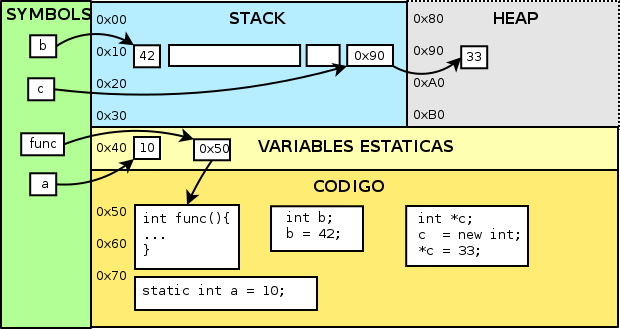
\includegraphics[width=.95\linewidth]{images/progmemoria}
%\end{center}
%}





\end{document}
